%%%%%%%%%%%%%%%%%%%%%%%%%%%%%%%%%%%%%%%%%%%%%%%%%%%%%%%%%%%%%%%%%%%%%%%%%%%%%%%%%%%
\section{Aim}
\label{sec:1aim}
%%%%%%%%%%%%%%%%%%%%%%%%%%%%%%%%%%%%%%%%%%%%%%%%%%%%%%%%%%%%%%%%%%%%%%%%%%%%%%%%%%%

Create a model of Londoners daily movements based upon the London Transport Demand Survey

%%%%%%%%%%%%%%%%%%%%%%%%%%%%%%%%%%%%%%%%%%%%%%%%%%%%%%%%%%%%%%%%%%%%%%%%%%%%%%%%%%%
\section{Objectives}
\label{sec:1objectives}
%%%%%%%%%%%%%%%%%%%%%%%%%%%%%%%%%%%%%%%%%%%%%%%%%%%%%%%%%%%%%%%%%%%%%%%%%%%%%%%%%%%

\begin{itemize}
\item Explore the LTDS dataset and identify key data
\item Move data from local Microsoft Access database into a PostgreSQL + PostGIS database
\item Clean data
\item Complete modal specific routing (interrogation, querying, storage) between origin and destinations
\item Quality check the routing results and do further data cleaning
\item Create and populate final dynamic location database table
\item Analysis of results
\end{itemize}

%%%%%%%%%%%%%%%%%%%%%%%%%%%%%%%%%%%%%%%%%%%%%%%%%%%%%%%%%%%%%%%%%%%%%%%%%%%%%%%%%%%
\section{Background}
\label{sec:1_background}

As was heavily discussed in Section \ref{sec:staticexposurehealth} many air quality exposure studies do not consider the movements of the subjects and/or to varying degrees other factors such as the temporal fluctuations in pollutant concentrations and levels of infiltration into micro-environments such as the home. The aim of this chapter was to process and characterise the LTDS prior to application to the hybrid exposure model. 

This was achieved by using the methods outlined in Sections \ref{sec:spatialdatabases} (Spatial databases), \ref{sec:gis} (GIS) and \ref{sec:routing} (Routing), and reconstructing the time-space location of the population of London on a minute-by-minute basis, using the LTDS dataset. This allowed interrogation of the data and such questions to be answered as; how much time do people spend indoors each day, and is there ethnic bias in the distance that people travel to work? To demonstrate the capacity of the model/dataset visualisations/maps of peoples routes were created and summary graphs of interesting information.

%%%%%%%%%%%%%%%%%%%%%%%%%%%%%%%%%
\section{Methods}
\label{sec:1_methods}

\subsection{Data Processing}
\label{sec:reconstruction_data_processing}

The LTDS comprised of around 58 tables of data stored in an Microsoft Access database. The majority of these tables were 'look-up' tables that store information that can be linked too from other tables e.g. the Stages table described the stages of trips that the subjects made, and had a column for transport mode which simply contains integers in the range 1-26. These integers needed cross-referencing against the Mode table to ascertain their meaning (1 = walk, 3 = car etc). This allows for more efficient storage of data, but made gaining a full understanding of the dataset and how tables linked together a lenghty process. The four key tables that were required were (as briefly discussed in Section \ref{sec:the_ltds}) the Household, Person, Trip and Stage tables. Within each table there were columns that were more or less useful than others.  Table \ref{tab:key_ltds_fields} below lists some of the more important and useful ones:

\newpage

\begin{center}
\begin{table}[h!]
    \begin{tabular}{ | p{2.2cm} | p{12cm} |}
    \hline
    \textbf{Table} & \textbf{Key fields} \\ \hline
    \multirow{2}{*}{Household} & hhid: household id \\
     & hhaboro: Household Borough \\
     & htdate: Date house survey refers too \\
     & hincomeei: Household income \\
     & hhose and hhosn: easting and northing of household \\ 
     & householddatatime: This column was created and populated with a full time-stamp \\ \hline
   \multirow{2}{*}{Person} & phid: Person id \\
     & phid: Household id of person \\
     & ppiwt: Expansion factor of person \\
     & psexi: Person gender \\
     & pagei: Person age \\
     & pegroup: Person ethnic group \\
     & pegroup: Person ethnic group \\
     & pseg: Person socio-economic group \\
     & pnotrips: Number of trips person takes in survey 24 hours \\ \hline
     \multirow{2}{*}{Trip} & ttid: Trip id \\
     & tpid: id of person doing the trip \\
     & tstagesn: Number of stages in the trip  \\
     & tdpurp: Destination purpose of trip \\
     & tstime: Trip start time \\
     & tetime: Trip end time \\
     & toose and toosn: Trip origin (OSGB36 Easting and Northing) \\
     & tdose and tdosn: Trip destination (OSGB36 Easting and Northing) \\
     & tdurn: Duration of trip \\ 
     & departuretime: This column was created and populated with a full time--stamp of the trip departure time \\
     & arrivaltime: This column was created and populated with a full time--stamp of the trip arrival time \\ \hline
    \multirow{2}{*}{Stage} & ssid: Stage id \\
     & stid: Trip id \\
     & smode5y: Stage mode of transport \\
     & soose and soosn: Stage origin (OSGB36 Easting and Northing) \\
     & sdose and sdosn: Stage destination (OSGB36 Easting and Northing) \\
     & sdurn: Duration of trip (minutes) \\
     & stagedeparturetime: This column was created and populated with a full time--stamp of the stage departure time \\
     & stagearrivaltime: This column was created and populated with a full time--stamp of the stage arrival time \\ \hline
    \end{tabular}
    \caption{Key LTDS fields}
    \label{tab:key_ltds_fields}
\end{table}
\end{center}

The tables listed above were exported as CSV files and then imported into a PostgreSQL installation on a virtual Ubuntu machine. PostGIS was then added to the PostgreSQL installation. SQL scripts were ran to create full time-stamp columns in the Household, Trip and Stage tables rather than use the format that the data was stored in e.g. dates were stored in the Household table in the form '20060221' (meaning 2006-02-21) and times in the Trips table as '730' (meaning 07:30) which made performing temporal queries on them difficult. Further complications arose in the Trips and Stages tables as the survey period begins and ends at 4am (or once the persons final trip was completed). So times in the Trips table showed as, for instance ,'300' which meant 3am, however that actually meant 3am on the morning of the day after the survey date, rather than the survey date itself. Another factor was that the stages table did not contain any stage departure times or stage arrival times, only the duration of each stage. Therefore the stages table needed cross-referencing against the trip table and then summing incrementally by stage id in order to calculate the correct stage departure and arrival times (and then extensively checking).

\subsection{Data cleaning}
\label{sec:reconstruction_data_cleaning}

Data cleaning was required throughout the methods, however is briefly mentioned here. A number of different processes were required, a few of which are listed as bullet-points below. It should be noted that an early decision was taken whereby if any data linked to a Person was clearly incorrect, or not recorded properly, then that person was removed from the dataset entirely (by creation of a column in the Person table titled 'badflag' and then entering the reason the person was removed). For example if a person had a stage which started 15 minutes before the next noted stage began, that person was removed rather than just a correction of the data (in this case because it would be difficult to know stage which to correct). Removal of records from the dataset occurred in the following situations:

\begin{itemize}
\item Trip start and end times were mis-aligned
\item Stage start and end times were mis-aligned
\item Stage transport mode was missing or refused
\item Key demographic data was missing or refused
\item Stage start and end locations were mis-aligned with the next or previous trip by greater than 80 metres
\item LTDS respondent did not live in London (the survey stretches just beyond the London Borough boundary)
\item Location of stage start or stage end were missing.
\item Transport mode was not available via a known API e.g. Plane or a bus journey outside of London
\end{itemize}

To ensure that removal of subjects from the dataset had not compromised the overall structure and statistical strength of the data (and therefore made using the weighting factors to scale the data unsuitable), t-test and Wilcoxon–Mann–Whitney tests were performed to compare the original data, and this subset of data. No statistical significance was found when comparing age, Borough of residence, ethnicity, income, sex, distances travelled each day, or the amount of time in transport. The final dataset to be used was therefore judged as suitable for purpose.

\subsection{Mode-specific routing}
\label{sec:reconstruction_mode_routing}

To calculate the locations of the subjects while they were travelling between locations the stages table of the LTDS was used, specifically the start easting and northing, the destination easting and northing, the transport mode, and the stage departure time (if allowed as an input by the API). These columns were extracted from the database directly into R using the RPostgreSQL extension and stored in an R dataframe. These details were then formed into URL requests and sent to the routing APIs by R. A small extract of the large XML file that is received in response to a request to the TfL Journey Planner API is shown in Figure \ref{fig:tfl_response_example}. This was parsed using the RJSONIO and XML packages, and the route between the two locations extracted and stored (and then decoded in the case of Google). The route was then formed into a linestring data type (which PostGIS can store as a spatial object) and entered back into the database as the route taken between the coordinates in an extra column called 'the\textunderscore geom'.

\begin{figure}[H]
\centering
\includegraphics[scale=0.9]{tfl_response_example}
\caption{An example of an XML response from the TfL API}
\label{fig:tfl_response_example}
\end{figure}

Due to restrictions on usage limits, and the modes of transport that each API has available, different APIs were used for each transport mode in the LTDS (see Table \ref{tab:api_transport_modes}). Pre-processing was required to simplify the transport modes before this, for example the LTDS contains transport modes such as 'Car (passenger)', 'Taxi', 'Van (driver)', 'Van (passenger)' and 'Motorcycle (driver)' which were combined to the mode of 'car' given that the likely routes would be the same (and more importantly that the API did not have the ability to distinguish between them as an input).

\begin{table}[H]
\hspace*{-.1cm}%
    \begin{tabular}{@{} | R{5cm} | R{8cm} |@{}}
    \hline 
     \bfseries{LTDS Transport Mode} & \bfseries{API} \\ \hline
     Walking & OpenRouteService (\url{www.openrouteservice.org}) \\ \hline
    Cycling & Google Directions \\ \hline
    Train, Overground, Underground, Docklands Light Railway, Bus & Transport for London Journey Planner \\ \hline
    Car & Project OSRM API (\url{www.project-osrm.org}) \\ \hline
    \end{tabular}\hspace*{-2cm}%%stop complaining
\caption{APIs used for each LTDS transport mode}
\label{tab:api_transport_modes}

\end{table}

The cleaned data contained 45,079 people, who took 98,770 trips during the day of the survey. Each trip consisted of multiple stages that needed routing independently, totally 340,754. These 340,000 routes were stored as linestrings in the PostGIS database next to the id (ssid) of the stage.

\subsection{Quality checking}
\label{sec:reconstruction_quality_checking}

Spatial cleaning of the routes was now performed. This is discussed earlier in Section \ref{sec:reconstruction_data_cleaning}. It primarily consisted of error-checking of the routes that had been obtained from the APIs by making visualisation of the transport modes to manually identify large errors e.g. were there any tube journeys recorded as being in Scotland, or a taxi journey accross the Irish sea. The results of the underground and Docklands Light Railway (DLR) routing are shown in \ref{fig:underground_routing} below.

\begin{landscape}

\begin{figure}[H]
\centering
\frame{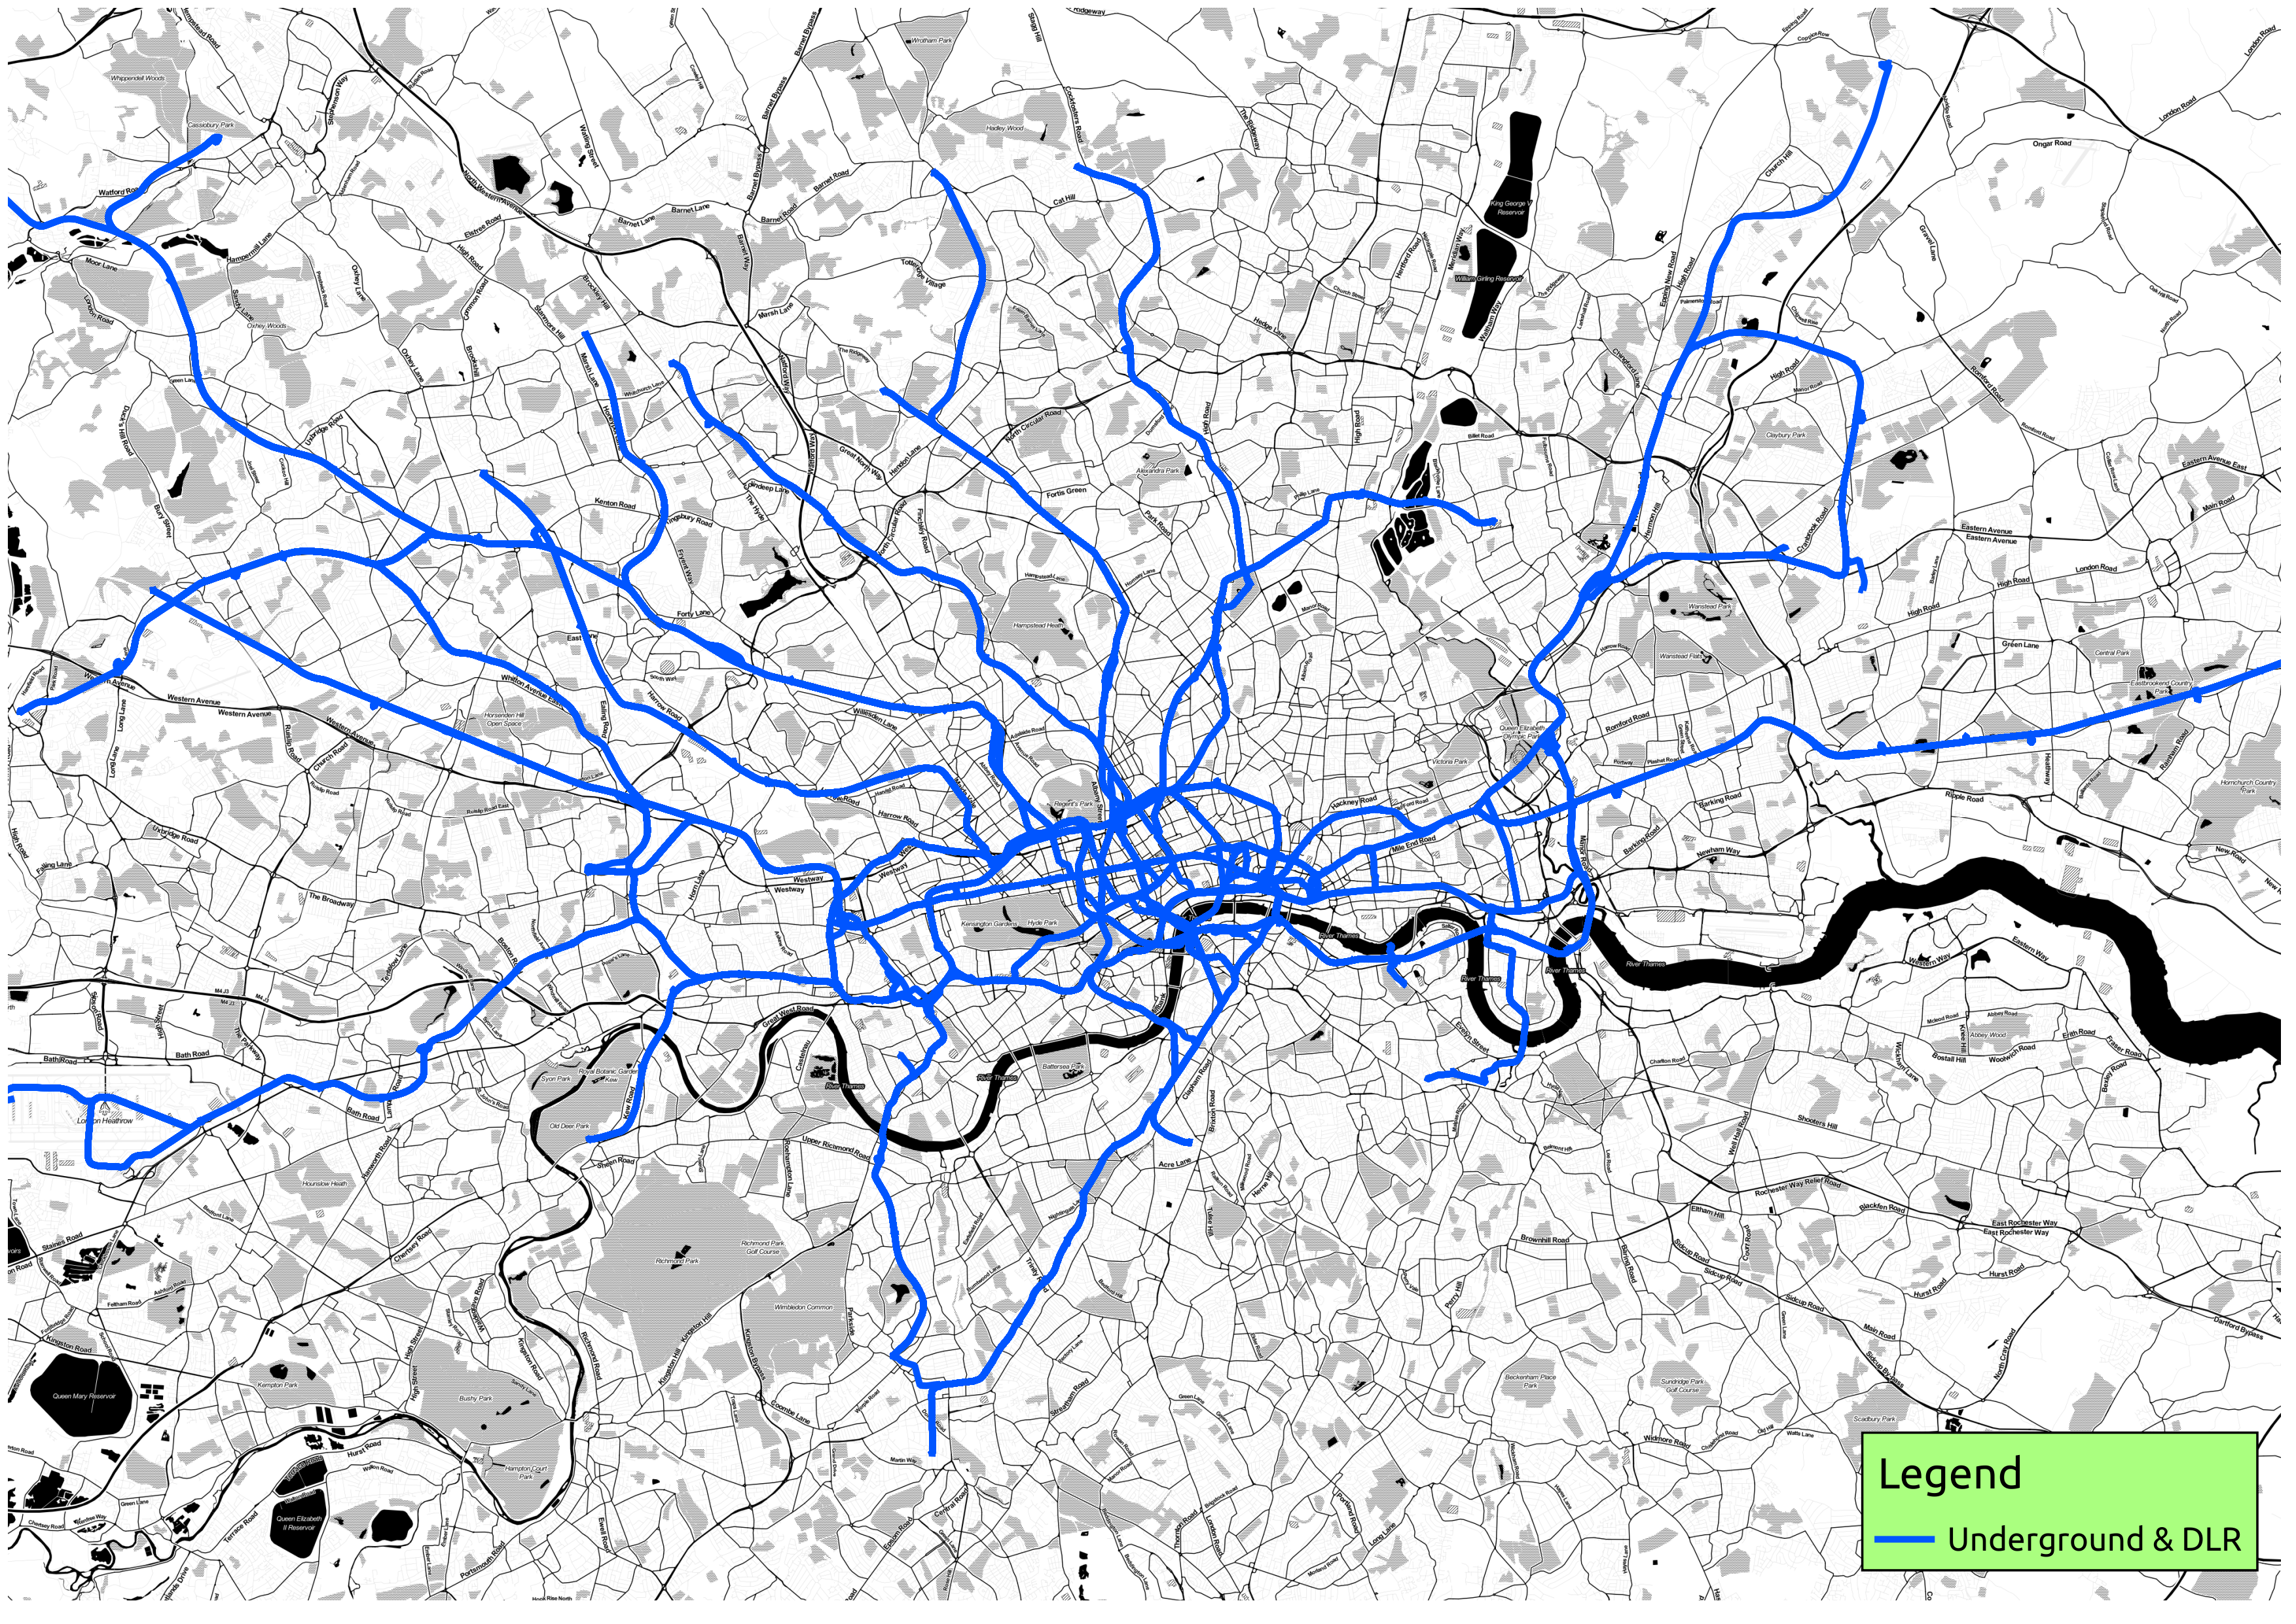
\includegraphics[scale=0.65]{underground_routing}}
\caption{A visual check that the underground routes actually are on the underground lines}
\label{fig:underground_routing}
\end{figure}

\end{landscape}

\subsection{Data manipulation}
\label{sec:reconstruction_data_manipulation}

A 'base table' for each subject in the cleaned and routed LTDS data (45,079) was now created (and named the hybrid\textunderscore location table). This table contained four columns, Person ID (ppid), Time (pointtime), Mode (mode) and Location (thegeom). A blank row for every minute of the subjects 24 hours was created (45,079 subjects, multiplied by 24 hours, multiplied by 60 minutes). The table was then populated with data from the Stage table, by taking the line-strings of each route and splitting them into minute-by-minute interval points using bespoke spatial interpolation SQL scripts, and then matching those points to the correct time in the new table. The mode and id of the stage were also copied over for ease of future reference. A graphic which attempts to demonstrate the premis behind the spatial interpolation method is shown below in \ref{fig:spatial_interpolation_example}.

\begin{figure}[H]
\centering
\includegraphics[scale=0.6]{spatial_interpolation_example}
\caption{The time and location between two known locations and times were calculated using custom-made SQL scripts and the spatial functions of PostGIS}
\label{fig:spatial_interpolation_example}
\end{figure}

Inbetween Trips subjects were presumed to be stationary and indoors at the final point recorded of the previous trip. At the start and end of days subjects locations were presumed to be the starting point of their first trip, and the ending location of their last trip respectively (and again, indoors). By doing this the location of the 45,079 people were calculated and stored on a minute-by-minute basis for 24 hours. An extract of the final table is shown below in \ref{fig:hybrid_location_table} (for reference mode 0 = indoors, 1 = walking, 3 = car).

\begin{figure}[H]
\centering
\frame{\includegraphics[scale=0.6]{hybrid_location_table}}
\caption{An example of data and structure in the hybrid location table}
\label{fig:hybrid_location_table}
\end{figure}

%%%%%%%%%%%%%%%%%%%%%%%%%%%%%%%%%
\section{Results}
\label{sec:reconstruction_results}

The hybrid location table was used to examine the movements of the subjects of the LTDS on a fine temporal and spatial scale. The data was explored to better understand the detail available, to check that it was suitable for use as the basis of a dynamic exposure model, and to see whether there were any interesting results already present before air quality was considered.

\subsection{Visual inspection of individuals}
\label{sec:visual_inspection_of_individuals}

Before starting to summarise data and look for patterns in large groups of people, Figures \ref{fig:routed_results_example} and \ref{fig:routed_results_example2} were created and show the results of two randomly selected individuals from the dataset. The first (\ref{fig:routed_results_example}) shows a fairly simple reconstructed day. The Person made two car journeys around the local neighbourhood, as well as one walking trip to a few streets away. Other than visiting those three local locations, they spent their time at home. The second (\ref{fig:routed_results_example2}) shows a much more complicated picture. The individual lives near Norbiton. In the morning they walked to Norbiton station, took a train to Waterloo, and then caught a bus to Clerkenwell (presumably for work). At lunchtime they walked around the local neighbourhood (buying lunch?). At 20:13 they took a taxi back to Waterloo, where they got a train back to Norbiton, and walked home from the station to their house.

\begin{landscape}

\begin{figure}[H]
\centering
\frame{\includegraphics[scale=0.65]{routed_results_example}}
\caption{Example one of the reconstruction of a subjects day}
\label{fig:routed_results_example}
\end{figure}

\newpage

\begin{figure}[H]
\centering
\frame{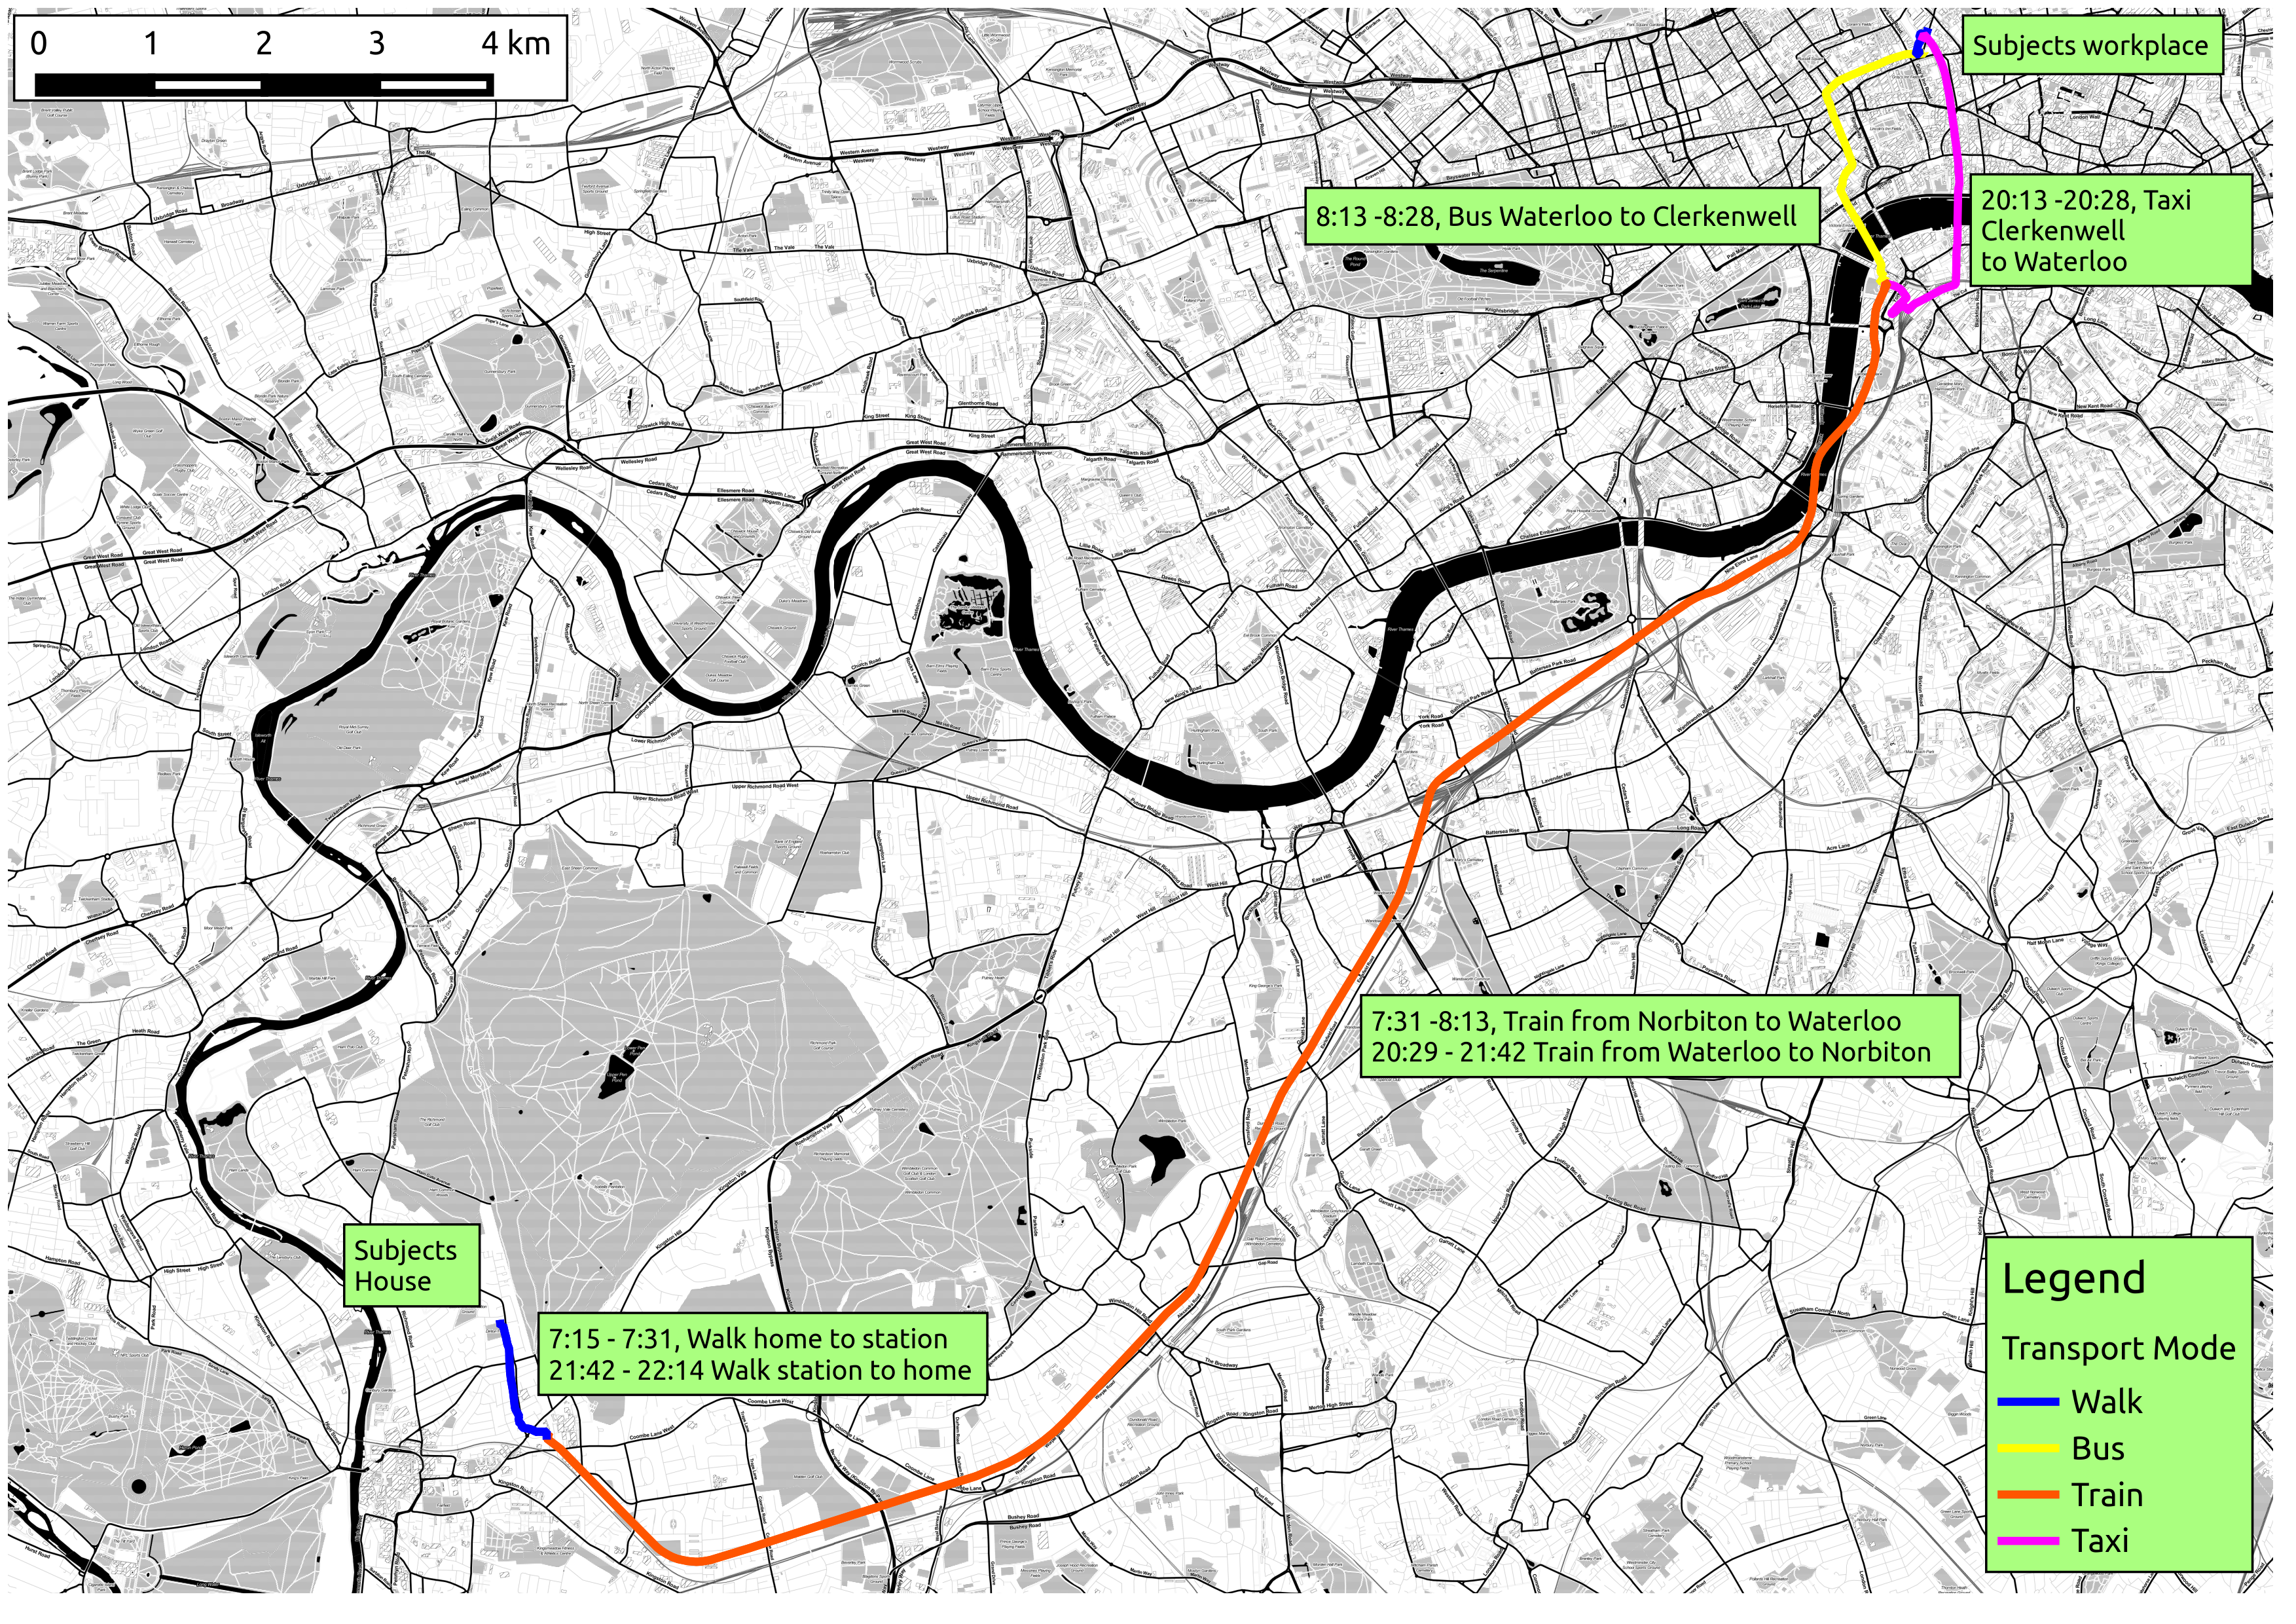
\includegraphics[scale=0.65]{routed_results_example2}}
\caption{Example two of the reconstruction of a subjects day}
\label{fig:routed_results_example2}
\end{figure}

\end{landscape}

\subsection{Journey start and end times}
\label{sec:journey_start_and_end_times}

By grouping the start times of the stages by hour, and then summarising by the number of stages within that hour, a histogram of journey start times was created (Figure \ref{fig:when_people_start_trips}).

\begin{figure}[H]
\centering
\includegraphics[scale=0.48]{when_people_start_trips}
\caption{Histogram of when the population of London start trips}
\label{fig:when_people_start_trips}
\end{figure}

A similar method was also used for the ending times (Figure \ref{fig:when_people_end_trips}).

\begin{figure}[H]
\centering
\includegraphics[scale=0.48]{when_people_end_trips}
\caption{Histogram of when the population of London end trips}
\label{fig:when_people_end_trips}
\end{figure}

Figures \ref{fig:when_people_start_trips} and \ref{fig:when_people_end_trips} show peaks of travel around peak travel times that might be expected in the morning and evening rush hours, however it is interesting to note that considerable travel occurs during the day (although at this stage the data is not split by specific days, so this may be influenced by travel on a Saturday and Sunday). It was also interesting to see how trips during the evening (4pm-8pm) are much more dispersed than in the morning, suggesting that people tend to leave work over a longer time-frame than when they start work. 

\subsection{Journey distances by sex}
\label{sec:journey_distances_by_sex}

By summing the total distance travelled by each person over 24 hours, and then grouping by gender, graph \ref{fig:mean_distance_by_sex} shows differences in total travel distance.

\begin{figure}[H]
\centering
\includegraphics[scale=0.5]{mean_distance_by_sex}
\caption{Boxplot of distances travelled, by gender (outliers \textgreater 100 km omitted for clarity, red line links each mean)}
\label{fig:mean_distance_by_sex}
\end{figure}

Although the difference was not huge (Male mean of 18.28 km, Female mean of 13.89 km), there was a significant difference (using a t-test) between the kilometres that each gender travels in a day. Whether this is because women stay at home more than me, or whether the journeys that men are required to do during their day take them further was not clear (but could be investigated further as the dataset contains a great deal of contextual information).

\subsection{Journey distances by income}
\label{sec:journey_distances_by_income}

A similar method was then used but the demographic of household income was used as the variable to be considered rather than gender (individual-level income variables were unfortunately not collected). The result is shown in Figure \ref{fig:mean_distance_by_income}.

\begin{figure}[H]
\centering
\includegraphics[scale=0.5]{mean_distance_by_income}
\caption{Boxplot of distances travelled by income group  (outliers \textgreater 100 km omitted for clarity, red line links each mean)}
\label{fig:mean_distance_by_income}
\end{figure}

Interestingly the dataset showned that subjects that live in households with a higher income actually travel further than households with a lower income level (albeit with a levelling off and even slight dip around the \textsterling75,000 mark).

\subsection{Journey distances by age group}
\label{sec:journey_distances_by_age_group}

Distance of travel by age group was now plotted in Figure \ref{fig:mean_distance_by_age}.

\begin{landscape}

\begin{figure}[H]
\centering
\includegraphics[scale=0.7]{mean_distance_by_age}
\caption{Mean distances travelled by age group (outliers \textgreater 100 km omitted for clarity, red line links each mean)}
\label{fig:mean_distance_by_age}
\end{figure}

\end{landscape}

Figure \ref{fig:mean_distance_by_age} showed a clear rise in the distance that people travel each day as they get into their late teens, which then becomes fairly steady until mid-50s at which point the distances start to decline again. That said, a clear cut-off was not visible. The gradient of the slops between 60 and 90 is much more steady that at the other end of the age range, perhaps showing that the ages that people retire are more dispersed than the ages at which people start work.

\subsection{Journey distances by Borough of residence}
\label{sec:journey_distances_by_borough_of_residence}

The distances that the people of London travel, depending on their Borough of residence, was now considered. The centre of London was defined (the monument outside of Charing Cross station) and then the distance between this point and the centroid of each London Borough was calculated (Figure \ref{fig:borough_centroids}). Figure \ref{fig:mean_distance_by_borough} was then created, with the Boroughs ordered by this distance metric i.e. the centroid of the City of London is the closest Borough centroid to Charing Cross, so was plotted first. This ordering was undertaken as I theorised that individuals living nearer the centre of London would spend less time travelling than those in outer London.

\begin{figure}[H]
\centering
\frame{\includegraphics[scale=0.5]{borough_centroids}}
\caption{Calculating Borough centroids to Charing Cross}
\label{fig:borough_centroids}
\end{figure}

\begin{landscape}

\begin{figure}[H]
\centering
\includegraphics[scale=0.7]{mean_distance_by_borough}
\caption{Mean distances travelled by Borough of residence}
\label{fig:mean_distance_by_borough}
\end{figure}

\end{landscape}

There did not appear to be any clear pattern between where people live and the distance that they travel each day. As the Boroughs were plotted in order, if it was true that people living in outer London Boroughs travel more, then the medians and means of the graph should rise from left (closest to centre of London) to right (furthest from centre of London). The Borough with the lowest mean was actually found to be Greenwich, perhaps reflecting that the people who live in Greenwich tend to work more locally (this could be investigated using the dataset). The boroughs with the highest mean travelling distance were Havering, Richmond and Merton.

\subsection{Transport mode choice by age group}
\label{sec:transport_mode_choice_by_age_group}

Focusing now on transport mode choice, the percentage of time that each person spends within each micro-environment, namely bus, car, cycling, train, underground and walking, was calculated. The indoors environment was found to be very dominant i.e. people spent most of their days indoors. For clarity of visualisation, the indoor environment was removed, and the remaining ones plotted by age bracket (Figure \ref{fig:age_barplots_time_transport}).

\begin{figure}[H]
\centering
\includegraphics[scale=0.7]{age_barplots_time_transport}
\caption{Percent of typical day using transport modes by income bracket}
\label{fig:age_barplots_time_transport}
\end{figure}

This graph agrees well with Figure \ref{fig:mean_distance_by_age} (travel distances by age group) which showed a bell-curve like distribution, with a leaning towards the upper age groups. Additionally however Figure \ref{fig:age_barplots_time_transport} shows how use of transport modes changes with age. Except for the 0--10 age group, bus transport is used the same amount by all ages. Walking has a similar pattern, being used frequently by people even up to the ages of 80 and above. Cycling is popular with the 20 to 60 year old's, but then hardly used by people older than that. The underground results are interesting in that it is almost never used by anyone in the 0-10 age bracket, or the 80+ age bracket. Despite free travel being granted to people in those age groups.

\subsection{Time near residence}
\label{sec:time_near_residence}

One of the main motivations behind this research was to examine where people spend time, and therefore accumulate their exposure, and whether using address or postcodes (or dynamic methods) for exposure assessment was valid. To examine this, a 1 km buffer was created around each residents recorded residential address (example shown in Figure \ref{fig:one_km_buffer_house}).

\begin{figure}[H]
\centering
\includegraphics[scale=0.6]{one_km_buffer_house}
\caption{Example of a 1 km buffer around residential address}
\label{fig:one_km_buffer_house}
\end{figure}

Then the percent of time that each occupant of each house spends within that buffer was calculated. The results are shown in Figure \ref{fig:time_with_one_km_home_by_age}.

\begin{landscape}

\begin{figure}[H]
\centering
\includegraphics[scale=0.9]{time_with_one_km_home_by_age}
\caption{Boxplot of percent of time within 1 km of home address, means shown by red line}
\label{fig:time_with_one_km_home_by_age}
\end{figure}

\end{landscape}

Figure \ref{fig:time_with_one_km_home_by_age} shows an interesting pattern of time spent within subjects local neighbourhoods varying by age group. Considering the mean line (red), time spent at home hovers between the 70\% and 80\% mark with some small variation up and down between the ages of 5 and 60. From age 60 onwards the time spent within the local neighbourhood steadily increases to 90\% by age 70, and mid 90s from there onwards (with a sudden dip in the 98 and 99 year olds, however this seems likely to be due to small numbers of subjects of this age who happened to be quite active on the day of the survey).

For illustrative purposes three simple animations of the data--set were made. The first two using the QGIS TimeManager plug-in, and the third using javascript. They can be viewed online at the following URLs:

\begin{itemize}
\item A webpage with an interactive slider, whereby the user can view the time--activity points of the trips the subjects of the LTDS make, on a minute by minute basis, with the points colour-coded according to the mode at that point--time:
\begin{itemize}
\item \url{http://www.londonair.org.uk/research/dynamic_london/mode_animation.html}
\end{itemize}
\item An animated GIF file of the movements of the LTDS, clipped to show specifically London
\begin{itemize}
\item \url{http://www.londonair.org.uk/research/ltds_uk/traffic_london.gif}
\end{itemize}
\item An animated GIF file of the movements of the LTDS, showing the whole of the UK
\begin{itemize}
\item \url{http://www.londonair.org.uk/research/ltds_uk/traffic_uk.gif}
\end{itemize}
\end{itemize}

These illustrations allow a much better understanding of the data--set than was possible before. Instead of rows of an database, the data can be viewed and understood. When used in presentations to colleagues and external stakeholders (such as the TfL staff who collect the LTDS data), it was particularly useful in helping them become more familiar with the results of the process. Particularly interesting to note in the animations is the spatial distribution of the LTDS subjects, with their movements on the day of the survey clearly not limited to the geographical area of London (and thus justifying the need for a UK-wide CMAQ model of air quality concentrations). Also the number of people who travel from London to outside of London for work or otherwise.

%%%%%%%%%%%%%%%%%%%%%%%%%%%%%%%%%
\section{Discussion}
\label{sec:1Discussion}

Generating or manipulating the LTDS with the methods and tools discussed in this chapter proved complicated, particularly in writing the SQL and R scripts to interrogate the APIs, and then the spatial and temporal interpolation techniques to re-define the data in the resolution required. However having initially attempted to build custom transport networks using PostGIS and PgRouting (the PostgreSQL extensions), the methods attempted were much more productive in that they allowed a far higher percentage of routes to be solved, and with much higher accuracy. 

The dataset that has been produced is, to my knowledge, unparalleled in this area of study. Few studies have produced similar datasets, a notable one being \cite{Dhondt2012} and their 5 million subjects in the 'FEATHERS' dataset, however the temporal resolution of that model was only hourly and the spatial resolution down to 16 km by 16 km zones of Flanders (Belgium) rather than exact coordinates. Conversely, it could be argued that the hybrid\textunderscore location table actually be more highly resolved that it is. Time intervals of one-minute were chosen for convenience, when 30 seconds or even 1 second could have been used. However this seemed the most sensible choice on the basis that the dataset is already very large. Further research to assess the impact of perhaps changing to 30 second intervals could be worthwhile. The linked demographic data to the people and households of this data was also very useful in examining travelling patterns and mobility by different characteristics, which has been done in many studies before however normally by using crude measures such as euclidean distances between households and recorded workplaces, rather than by using routing solutions.

The limitations of this approach include the lack of finely-detailed control over the routing process and solution. Whilst most of the APIs allowed for different transport modes to be selected, and some of them give options such as 'avoid major roads', they do not allow cost-factors to be dynamically assigned to roads or for the network to be manipulated such as removing specific routes from the choices available. Whilst not an issue at this stage of this research, a situation can be envisaged whereby low exposure routing would be desirable, and this will prove difficult. Similarly, there is currently no way of validating the routes that were chosen by the subjects, as being representative of the actual routes taken. For some transport modes this seems less of a worry than for others. A subject taking a tube from London Bridge to Elephant and Castle for example has very little choice of their route (without significantly adding time to their journey), and much would be the same for other journeys using public transport. Private modes such as driving and walking would be less certain, however the time taken for the route matches the time in the LTDS, so whilst small detours are possible, large detours are unlikely.

The way that time inbetween trips is considered might be leading to an over-estimation of the amount of time that subjects spend indoors each day. This is because when subjects finish trips the model presumes that they are then inside until the next trip begins. Time spent not travelling but in outdoor spaces, is therefore neglected (for example in a park). Intersecting an Ordnance Survey land-use map with the dataset could lead to improvements in this area of the model. Further efforts could also be made to 'recover' discarded data which was removed in the data-cleaning process, for example subjects with miss-aligned trip start and end times were removed, but further investigation may have been able to resolve these issues.

Going forward, this dataset will now be referred to for simplicity as the LTDS-Expanded dataset, or the LTDS-X for short.  Specifically, the dataset created (expanded) by processing of the original LTDS data through routing algorithms and GIS.

%%%%%%%%%%%%%%%%%%%%%%%%%%%%%%%%%
\section{Conclusions}
\label{sec:1conclusions}

The aim of this research was to process and characterise the LTDS to create a new data--set that can be used as an input for a hybrid exposure model. Spatially-enabled databases with custom scripts were wrote to do this, R was used as an interface with various APIs, and the 'hybrid\textunderscore location' table was created successfully. Extensive quality checking and data cleaning was undertaken. The final data-set allows interrogation of the daily activities of 6.8 million people in London, which can be interrogated on a fine spatial and temporal detail, aswell as by various demographics. The main findings from this data--set were as follows:

\begin{itemize}
\item There are peaks in travel between 8am and 10am in the morning, and between 5pm and 6pm in the evening (As would be expected), however substantial travel also occurs between those hours.
\item Men travel more each day than women (mean of 18.28 km, compared to women with 13.89 km).
\item Households with a higher average annual income, are inhabited by people who travel more than households with a lower average annual income.
\item The distances that people travel each day increases as they get older, peaking around the ages of 38-42. It then steadily declines, however much more gradually than it rose. By late 80s, people travel very little.
\item There appears to be no pattern to where people live compared to the distances they travel each day
\item The amount of time that people spend in transport each day peaks in the 30-50 age categories.
\item Car use is the most popular form of transport amongst all age groups over 20 (until that point walking is the most popular). Walking is the second most popular, followed by the London Underground.
\item People over 80 rarely use the London Underground.
\item The amount of time that people spend within 1 km of their home, when analysed by age group, has a similar but slightly different pattern as the distance that people travel. Between the ages of 5 and 20, the mean is around 77\%, which then drops to the low 70\% mark for people aged 20 to late 50s. From 60 onwards, the time at home gradually increases up to high 80s.
\end{itemize}

This initial exploration and validation of the key characteristics of the data were important to confirm that it was suitable for use in further research. It will now be used as the main input for a hybrid exposure model to estimate subjects exposure to air pollution. 